\subsection{Формальная постановка задачи мониторинга системы}
\label{subsec:spec:DDMS:FormalTask}
Введём следующие обозначения:
\begin{description}
	\item[$M$]~---~дискретно-непрерывное пространство, имеющее $p$ непрерывных и $q$ дискретных измерений;
	\item[$R=\left\{R_1,R_2,\dots,R_n\right\} \in M$]~---~множество режимов работы системы;
	\item[$T=\left\{x_1,x_2,\dots,x_m\right\} \in M$]~---~обучающая выборка;
	\item[$x=\left\{a_1,a_2,\dots,a_p,b_1,b_2,\dots,b_q\right\} \in M, a_i\in\mathbb{R}, b_i\in\mathbb{N}$]~---~элемент обучающей выборки;
	\item[$\theta=\left\{\tilde{a}_1,\tilde{a}_2,\dots,\tilde{a}_p,\tilde{b}_1,\tilde{b}_2,\dots,\tilde{b}_q\right\} \in M, \tilde{a}_i\in\mathbb{R}, \tilde{b}_i\in\mathbb{N}$]~---~входной вектор;
	\item[$\Omega=\left\{\omega_1,\omega_2,\dots,\omega_{p+q}\right\}$]~---~вектор весов.
\end{description}

Необходимо отметить, что некоторые значения в векторах могут отсутствовать.
%\subsubsection{Определения}

Даны $n$ обучающих выборок $T_1\in R_1, T_2\in R_2,\dots, T_n\in R_n$ различной длины, содержащие $m_i$ элементов каждая, где $i$~---~номер режима работы системы. Дан вектор $\Omega$, содержащий веса, соответствующие важности каждого параметра системы. Дан входной вектор $\theta$.

Необходимо определить, принадлежит ли $\theta$ к $R$; если $\theta \in R$, то определить, в каком именно подмножестве $R_i\in R$ находится $\theta$. Если же $\theta \notin R$, найти численную меру $\lambda \in \mathbb{R}_{\geq 0}$, показывающую отклонение $\theta$ от $R$.

\subsection{Описание метода}
Предложенный ниже метод относится к методам, основанным на измерении расстояний между точками (distance-based). Поэтому для работы метода необходимо определить взвешенную метрику $d(x,y,\Omega)$ на пространстве $M$. В качестве такой метрики может выступать комбинация Евклидова расстояния~\eqref{eq:spec:DDMS:EuclidDistance} для непрерывных и функции отличия~\eqref{eq:spec:DDMS:DiffDistance} для дискретных переменных. Подобная метрика, определённая на пространстве $M$, показана в формуле~\eqref{eq:spec:DDMS:Distance}. В случае отсутствия значения прибавляется только вес данного параметра.

\begin{subequations}
\begin{equation} \label{eq:spec:DDMS:EuclidDistance}
D_E(x,y) = \sqrt{\sum_{i=1}^{n} \left(x_i - y_i\right)^2}
\end{equation}
\begin{equation} \label{eq:spec:DDMS:DiffDistance}
D_{diff}(x,y) = 
\begin{cases} 
	0, & x=y \text{,} \\
	1, & x\neq y \\
\end{cases}
\end{equation}
\end{subequations}

\begin{equation} \label{eq:spec:DDMS:Distance}
d(x,y,\Omega) = \sqrt{\sum_{i=1}^{p} \left[\omega_i \left(a_i^{(x)} - a_i^{(y)}\right)^2\right]} + \sum_{j=1}^{q} 
\left[\begin{cases} 
	0, & b_j^{(x)}=b_j^{(y)} \text{,} \\
	\omega_{j+p}, & b_j^{(x)}\neq b_j^{(y)} \\
\end{cases}\right]
\end{equation}

Блок-схема процесса обучения метода представлена в приложении~\ref{app:DDMS:TrainingScheme}.

Обучение метода проходит в два этапа: подготовка данных и формирование базы режимов.

Пример единицы входных данных для метода представлен в таблице~\ref{tab:spec:DDMS:SampleVector}.

\begin{table}[h]
\caption{Пример единицы входных данных разрабатываемого метода}
\label{tab:spec:DDMS:SampleVector}

\begin{tabular}{|C{55pt}|C{70pt}|C{55pt}|C{70pt}|C{75pt}|C{75pt}|}
\hline
Давление A & Состояние клапана 1 & Давление B & Состояние клапана 2 & Температура 1 & Температура 2 \\
\hline
2857.2 & Закрыт & 1218.4 & Открыт & 49.8 & 37.6 \\
\hline
\end{tabular}
\end{table}

\subsubsection{Подготовка данных}
\label{subsubsec:spec:DDMS:Preparing}
Формат входных данных, показанный в таблице~\ref{tab:spec:DDMS:SampleVector}, может не соответствовать формату, описанному в подразделе~\ref{subsec:spec:DDMS:FormalTask}. Для этого необходимо сгруппировать параметры по своей природе (отдельно непрерывные и отдельно дискретные). Для каждого дискретного параметра составляется список возможных значений, в соответствие которым ставятся натуральные числа.

Так как элементы в векторах могут иметь различный масштаб, для корректного определения расстояния между двумя точками непрерывные значения векторов сначала необходимо нормализовать. Для этого может применяться как минимаксная нормализация~\eqref{eq:spec:DDMS:MinimaxNormalization}, так и нормализация с помощью стандартного отклонения~\eqref{eq:spec:DDMS:StandardNormalization}. Метод сохраняет характеристики, используемые при нормализации обучающих вбыорок (минимум, среднее значение и т.д.), для масштабирования входного вектора на стадии мониторинга.

\begin{subequations}
\begin{equation} \label{eq:spec:DDMS:MinimaxNormalization}
\hat{x} = \frac{x - \min(X)}{\max(X) - \min(X)}, x\in X
\end{equation}
\begin{equation} \label{eq:spec:DDMS:StandardNormalization}
\hat{x} = \frac{x - \bar{x}}{\sigma_x} \text{,}
\end{equation}
\end{subequations}
\begin{description}
	\item[где $\bar{x}$]~---~среднее значение;
	\item[$\sigma_x$]~---~стандартное отклонение.
\end{description}

Зачастую в обучающих выборках могут содержаться аномальные элементы (сбой в работе датчика, искажения в канале связи и т.д.). Для того, чтобы метод мог корректно обучаться, необходимо их исключить. Для этого на каждой выборке используется алгоритм Orca, описанный в подразделе~\ref{subsec:spec:Orca}. В качестве количества аномалий, которые необходимо найти, ему задаётся число элементов в выборке. С учётом этой особенности на выходе данный алгоритм выдаёт численную меру (степень) аномальности для каждого вектора. Далее применяется фильтр, который на основе этой численной меры для каждого вектора определяет, является ли вектор аномальным. Для этого могут использоваться как статистические (например, Гауссовый фильтр, считающий аномальными все векторы, численная мера для которых не укладывается в диапазон $[0, 3\sigma]$), так и пороговые фильтры (считающие аномальными векторы, численная мера которых выше определённой величины $\delta$). Выбранные фильтром аномалии удаляются из выборки.

Результатом данного этапа являются нормализованные выборки $\hat{T}_i\in \hat{T}$, $i\in \left[1,n\right]$, не содержащие аномалий. Пример элемента такой выборки представлен в таблице~\ref{tab:spec:DDMS:PreparedSampleVector}.

\begin{table}[h]
\caption{Пример подготовленной единицы входных данных разрабатываемого метода}
\label{tab:spec:DDMS:PreparedSampleVector}

\begin{tabular}{|C{40pt}|C{40pt}|C{40pt}|C{40pt}|C{30pt}|C{30pt}|}
\hline
$a_1$ & $a_2$ & $a_3$ & $a_4$ & $b_1$ & $b_2$ \\
\hline
0.91 & 0.38 & 0.85 & 0.64 & 0 & 1 \\
\hline
\end{tabular}
\end{table}

\subsubsection{Формирование базы режимов}
На данном этапе производится создание отдельной базы кластеров для каждого режима работы системы $R_i$, $i\in \left[1,n\right]$. Блок-схема процесса представлена в приложении~\ref{app:DDMS:ClusterDBScheme}.

Каждый кластер определяет диапазон допустимых значений для непрерывных переменных $\left(a_1,a_2,\dots,a_p\right)$ и список допустимых значений для каждой дискретной переменной из $\left(b_1,b_2,\dots,b_q\right)$. Пример такого кластера представлен в таблице~. Вектор верхней границы и вектор нижней границы в кластере могут быть представлены, как углы минимального ограничивающего прямоугольного параллелепипеда в $p$-мерном пространстве ($p$~---~число непрерывных переменных в векторе).

\begin{table}[h]
\caption{Пример кластера разрабатываемого метода}
\label{tab:spec:DDMS:SampleCluster}

\begin{tabular}{|C{75pt}|C{40pt}|C{40pt}|C{40pt}|C{40pt}|C{30pt}|C{30pt}|}
\cline{2-7}
\multicolumn{1}{c|}{} & $a_1$ & $a_2$ & $a_3$ & $a_4$ & $b_1$ & $b_2$ \\
\hline
Верхняя граница & 0.91 & 0.38 & 0.85 & 0.64 & -- & -- \\
\hline
Нижняя граница & 0.45 & 0.45 & 0.55 & 0.14 & -- & -- \\
\hline
Допустимые значения & -- & -- & -- & -- & 0, 1 & 1 \\
\hline
\end{tabular}
\end{table}

Метод последовательно обрабатывает все векторы из выборки $T_i\in R_i$. Процесс начинается с пустой базой кластеров. Первым вектором инициализируется начальный кластер (нижняя и верхняя граница этого кластера считаются равными вектору, в списки допустимых значений дискретных переменных добавляются значения дискретных переменных вектора). Каждый последующий вектор сравнивается со всеми кластерами в базе. Если вектор полностью находится в границах кластера, то метод переходит к следующему вектору в обучающей выборке. Если вектор не попал ни в один кластер, то измеряется расстояние $d_c(x,c,\Omega)$ между вектором и всеми кластерами в базе с целью нахождения наиболее близкого кластера. Вводится пороговое значние $\varepsilon$, заданное пользователем, которое определяет максимальное допустимое расстояние между вектором и кластером (размер окрестности кластера). Если $d_c(x,c,\Omega) \leq \varepsilon$, то вектор находится в окрестности кластера и может быть включён в него. При этом границы кластера расширяются, чтобы включить в себя вектор, а в списки допустимых значений дискретных переменных добавляются соответствующие значения элементов вектора. Если же $d_c(x,c,\Omega) > \varepsilon$, то формируется новый кластер, инициализирующийся этим вектором, и добавляется в базу. Процесс обучения повторяется до тех пор, пока не будет обработана вся обучающая выборка. Малое значение $\varepsilon$ приводит к созданию небольших по размеру кластеров, что обеспечивает более точный контроль, но значительно увеличивает размер базы знаний, делая невозможным мониторинг системы в реальном времени. Значение $\varepsilon$ может быть подобрано таким образом, чтобы обеспечить баланс между скоростью работы и точностью контроля.

Функция расстояния $d_c(x,c,\Omega)$ может быть определена различными способами, зависящими от точки в кластере, до которой измеряется расстояние. В отличие от метода IMS, описанного в подразделе\ref{subsec:spec:IMS}, использующего расстояние до центра кластера (рисунок~\ref{fig:spec:DDMS:KMeansDistance}), предлагается использовать расстояние до ближайшей точки кластера (рисунок~\ref{fig:spec:DDMS:NearestDistance}), обеспечивающее более точную оценку удалённости вектора от границ кластера.

\begin{figure}[h]
	\begin{subfigure}[b]{0.35\textwidth}
		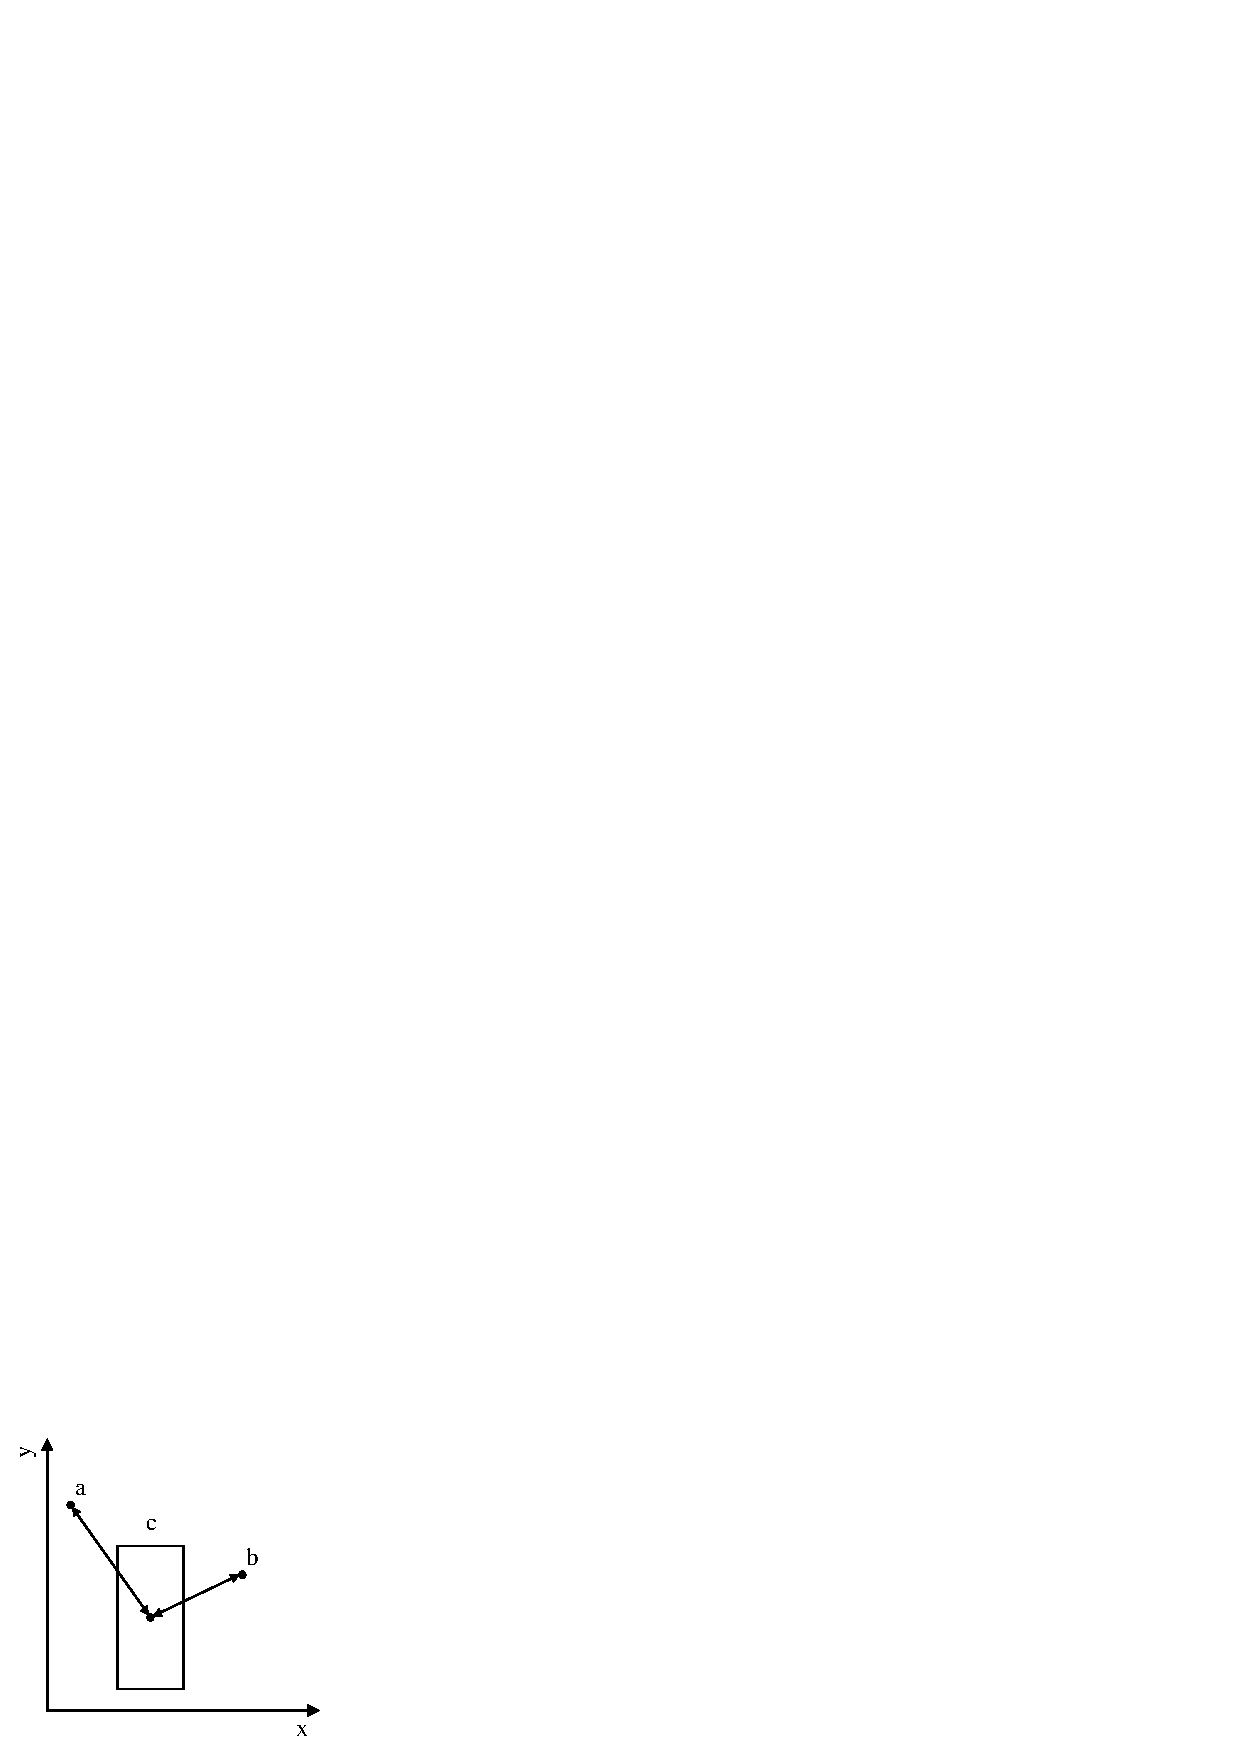
\includegraphics[width=\textwidth]{ddms_kmeans_distance}
		\caption{До центра кластера}
		\label{fig:spec:DDMS:KMeansDistance}
	\end{subfigure}
	\hspace{0.5cm}
	\begin{subfigure}[b]{0.35\textwidth}
		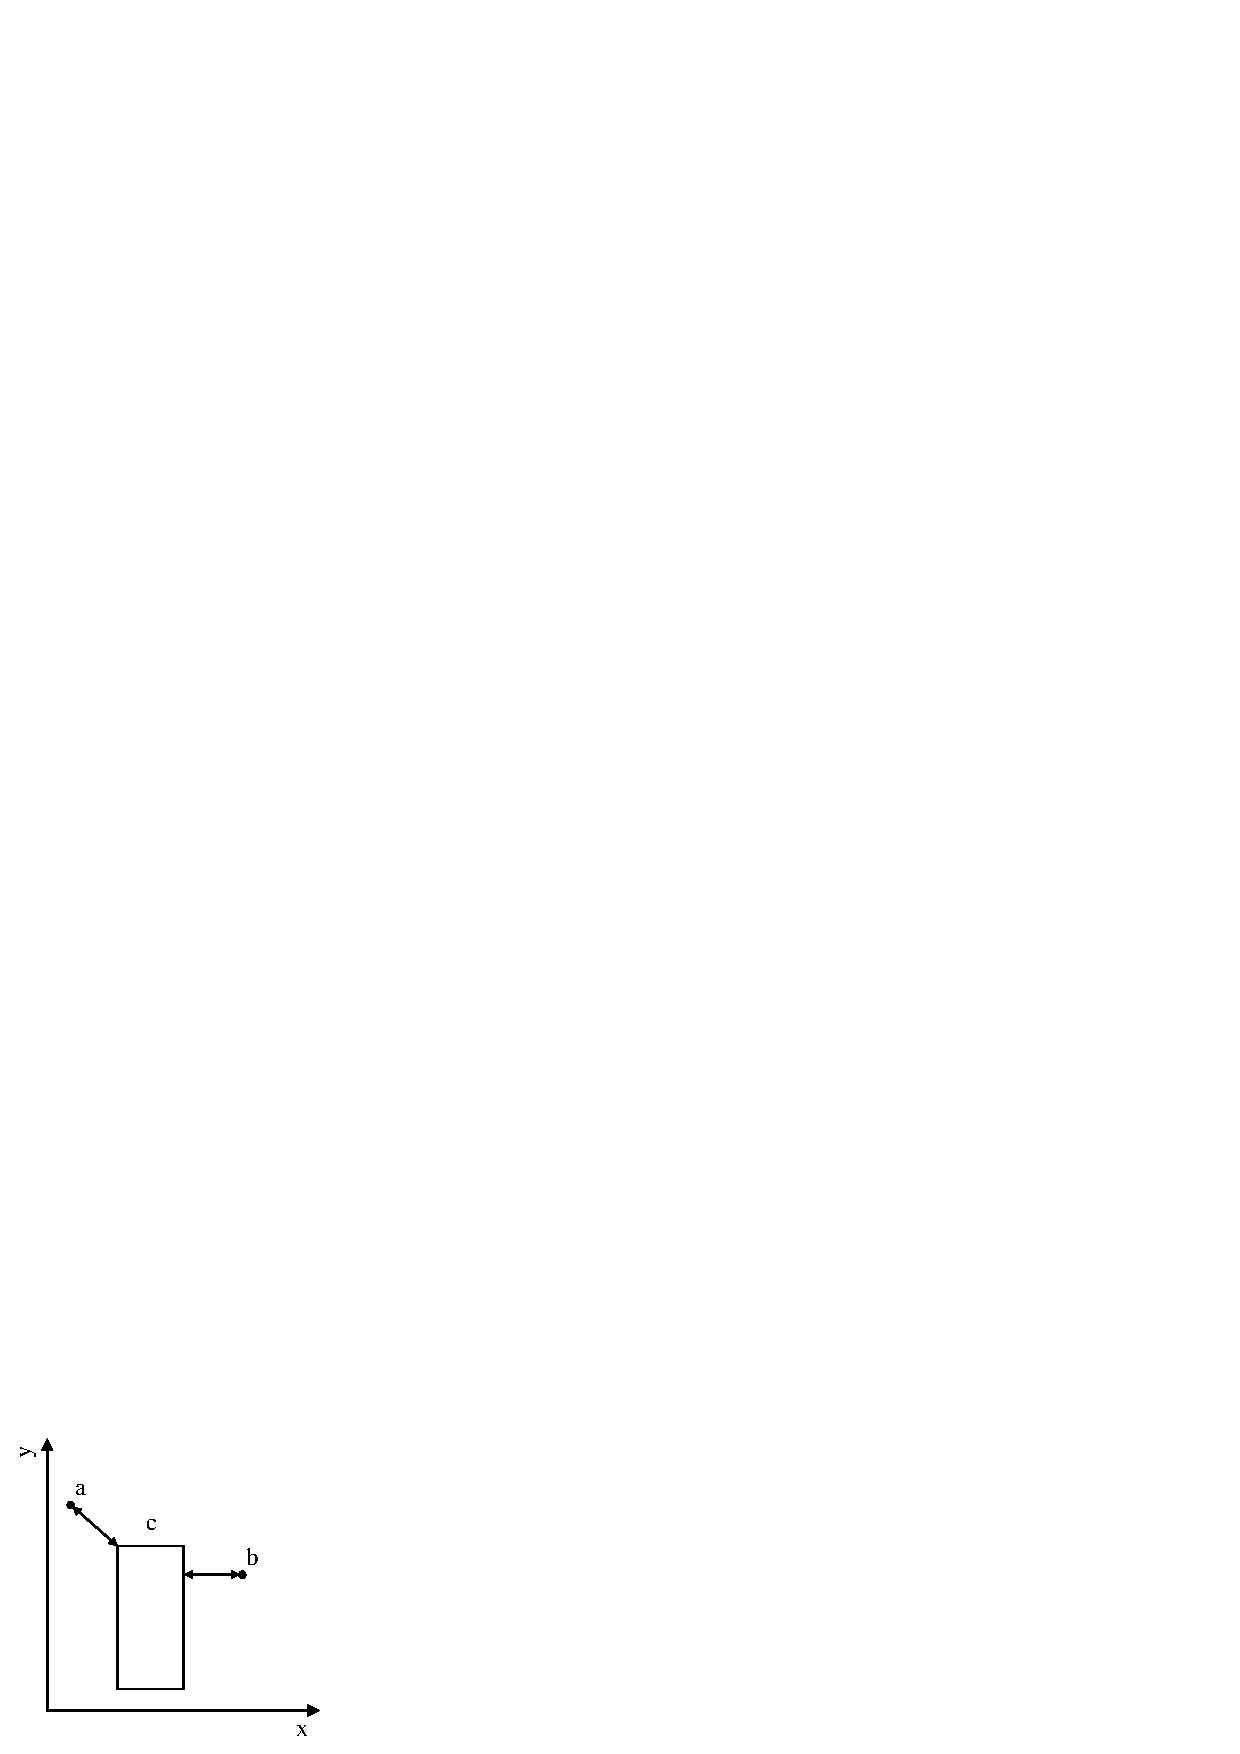
\includegraphics[width=\textwidth]{ddms_nearest_distance}
		\caption{До ближайшей точки кластера}
		\label{fig:spec:DDMS:NearestDistance}
	\end{subfigure}
	\caption{Виды расстояний от вектора до кластера}
\end{figure}

Результатом работы данного этапа является модель системы, состоящая из режимов, каждый из которых содержит базу кластеров. Структура модели показана на рисунке~\ref{fig:spec:DDMS:ModelStructure}.

\begin{figure}[h]
	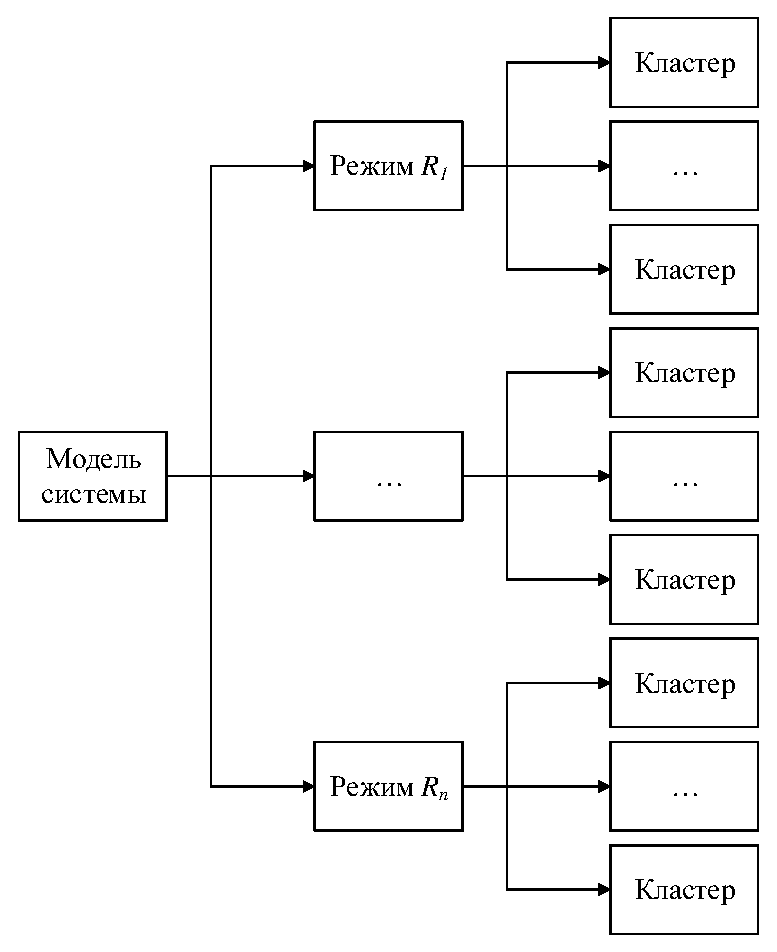
\includegraphics[height=0.45\textheight]{ddms_model_structure}
	\caption{Структура модели системы для разрабатываемого метода}
	\label{fig:spec:DDMS:ModelStructure}
\end{figure}

\subsubsection{Мониторинг состояния системы}
Для использования получившейся модели системы для мониторинга текущего состояния требуется получить из пришедшего вектора измерений входной вектор $\theta$ в формате, описанном в подразделе~\ref{subsec:spec:DDMS:FormalTask}, и нормализовать его. Для этого над вектором измерений производятся операции, описанные в пункте~\ref{subsubsec:spec:DDMS:Preparing}. Нормализация производится с использованием характеристик, сохранённых на аналогичном этапе при подготовке данных обучающих выборок.

Метод по очереди перебирает режимы и проверяет, находится ли входной вектор внутри одного из кластеров в базе режима. Если входной вектор попал внутрь кластера, то система работает в том режиме, к которому относится данный кластер. Иначе путём измерения расстояний $d_c(x,c,\Omega)$ от входного вектора до каждого кластера находится ближайший кластер. Если  $d_c(x,c,\Omega) \leq \varepsilon$, то вывод аналогичный с поправкой на то, что возможно отклонение от номинального поведения, поэтому метод даёт численную характеристику степени отклонения в виде расстояния $d_c(x,c,\Omega)$. В случае, когда $d_c(x,c,\Omega) > \varepsilon$ для всех кластеров во всех режимах, поведение системы считается аномальным; метод выводит ближайший режим и расстояние до него. Блок-схема данного процесса приведена в приложении~\ref{app:DDMS:MonitoringScheme}.